\chapter{Question 1}
\label{intro}

\textbf{Use D3 to visualize your Twitter followers.  Use my twitter account (``@phonedude \textunderscore mln'') if you do not have $>$= 50 followers.  For example, @hvdsomp follows me, as does @mart1nkle1n.  They also follow each other, so they would both have links to me and links to each other.}

\textbf{To see if two users follow each other, see: }
\url{https://dev.twitter.com/rest/reference/get/friendships/show}\\
\textbf{Attractiveness of the graph counts!  Nodes should be labeled (avatar images are even better), and edge types (follows, following) should be marked.}\\
\textbf{Note: for getting GitHub to serve HTML (and other media types), see:}
\url{http://stackoverflow.com/questions/6551446/can-i-run-html-files-directly-from-github-instead-of-just-viewing-their-source}\\
\textbf{Be sure to include the URI(s) for your D3 graph in your report. }

Following are the steps I have taken to the solve the problem:
\begin{itemize}
\item Using the Twitter API I extracted all my followers and stored `screen\textunderscore name', `name', `profile\textunderscore image\textunderscore url', and `index number' in a JSON file named as `nodesData'.
\item In function `links()' I stored the source and target nodes in a dictionary which gives the data for directed links. This code is listed in Listing \ref{lst:q1code1}.
\item I took the above generated `nodesData' file as input and obtained all possible pairs for my followers. This is stored in the file `sourceTarget'. 
\item For all these possible pairs I checked the existence of friendship between each other using `show\textunderscore friendship' API. 
\item This code is listed in Listing \ref{lst:q1code2} .
\item The final output Json is stored in `finalJsonData'. This data is taken as input for D3 code to generate a graph.
\item The Output of the graph is located in URI \url {http://bl.ocks.org/majetisiri/b0fe8280da899311640c}. The screen shot of the graph is illustrated in Figure \ref{fig:q1fig2}.
\begin{figure}[h!]
\begin{center}
\hspace*{-3cm} 
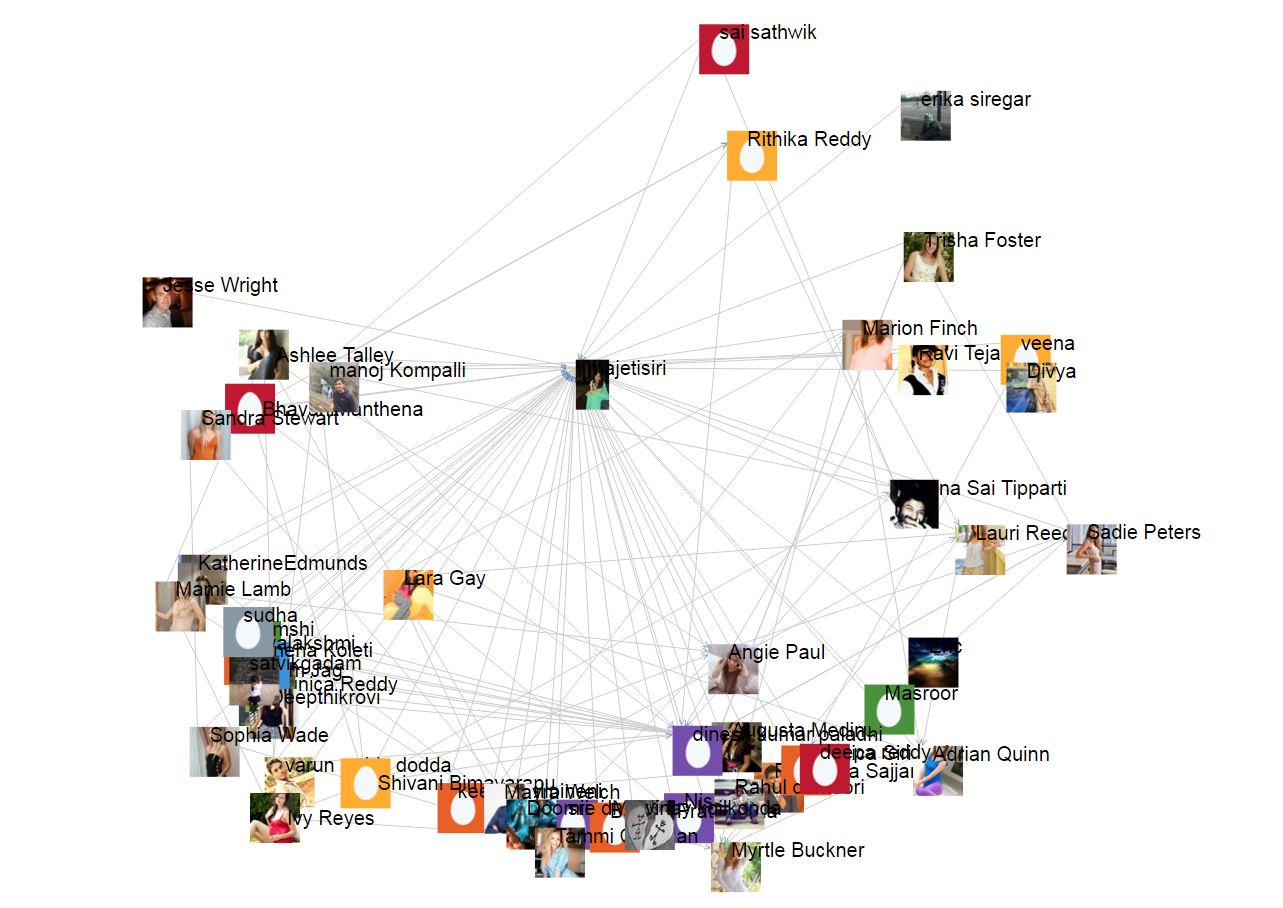
\includegraphics[scale=0.55, keepaspectratio=true]{figures/1.JPG}
\caption{Directed graph between me and my twitter followers including links between my followers if they have any}
\label{fig:q1fig2}
\end{center}
\end{figure}
\end{itemize}

\newpage
\textbf{Code Listing}
\sloppy
\lstinputlisting[language=Python,caption=Python code for getting my followers data,frame=single,breaklines=true,label=lst:q1code1, tabsize=2, captionpos=b,numbers=left,showspaces=false,showstringspaces=false,basicstyle=\footnotesize]{src/getFollowerLinksAndNodesData.py}

\newpage
\textbf{Code Listing}
\sloppy
\lstinputlisting[language=Python,caption=Python code for checking if friendship exists between my twitter followers ,frame=single,breaklines=true,label=lst:q1code2, tabsize=2, captionpos=b,numbers=left,showspaces=false,showstringspaces=false,basicstyle=\footnotesize]{src/checkFriendship.py}